%!TEX root = ../thesis.tex

\chapter{Introduction}


%%% This is just a dump of the introduction to paper, comments and all.
% Many phenomena across geophysical, biological and socio-economic applications can be modelled using a continuous-time dynamical system, i.e., an ordinary differential equation \cite[e.g.]{BrauerCastillo-Chavez_2012_MathematicalModelsPopulation,TelEtAl_2005_ChemicalBiologicalActivity,Wiggins_2005_DynamicalSystemsApproach}.
% Given initial values of a multi-dimensional state variable, such equations can be solved numerically to predict the state at future times.
% The governing dynamics may be specified using existing phenomenological models, but in modern applications these are usually supplemented or driven by observed data \cite{LawEtAl_2015_DataAssimilationMathematical,ReichCotter_2015_ProbabilisticForecastingBayesian}.
% % Standard examples include the modelling of weather using available data \cite{LawEtAl_2015_DataAssimilationMathematical,ReichCotter_2015_ProbabilisticForecastingBayesian}, and predicting concentrations of, for instance, temperature, pollutants or phytoplankton in the ocean using observed current velocity data \cite{AbascalEtAl_2009_ApplicationHFRadar,dOvidioEtAl_2010_FluidDynamicalNiches}.
% All methods using this approach have uncertainties in the model specification arising from a variety of sources \cite{FangEtAl_2020_DisentanglingResolutionPrecision}: the model not capturing all phenomena because of the inevitable lack of a complete understanding of all processes involved, errors in measured data, information only available on spatio-temporal grids (resolution error), etc.
% There are generally two manifestations of this uncertainty: in the initial state, and in the ongoing evolution of the model itself.
% In the absence of any other understanding of these multitudinous issues, a well-established way of tackling such uncertainties in the model is to think of these as stochastic \cite{BernerEtAl_2017_StochasticParameterizationNew,Oksendal_2003_StochasticDifferentialEquations}.
% Running many realisations of stochastic perturbations to the deterministic model can generate statistics to improve predictions and estimate their associated uncertainties \cite[e.g.]{BadzaEtAl_2023_HowSensitiveAre,Collins_2007_EnsemblesProbabilitiesNew}.
% However, in practice a very large number of simulations is necessary to generate convergent statistics \cite{FepponLermusiaux_2018_DynamicallyOrthogonalNumerical, Leutbecher_2019_EnsembleSizeHow}.
% Thus, numerically solving such stochastic systems -- potentially with data-based terms -- is often computationally expensive, and does not necessarily provide conceptual insight into how the model uncertainties affect predictions.
% Clearly, possessing a broader theoretical understanding of how stochastic terms impact continuous dynamical systems would be valuable.
Stochastic differential equations (SDEs) are a natural framework for introducing different sources of uncertainty %, as a noise process,
into the continuous time evolution of a variable \cite{Oksendal_2003_StochasticDifferentialEquations,SarkkaSolin_2019_AppliedStochasticDifferential,KallianpurSundar_2014_StochasticAnalysisDiffusion}.
Generally, in modelling situations the dynamics are highly nonlinear and one expects the noise to be multiplicative (i.e. vary with state), e.g. in atmospheric \cite{SuraEtAl_2005_MultiplicativeNoiseNonGaussianity,Sura_2003_StochasticAnalysisSouthern} and oceanic \cite{KamenkovichEtAl_2015_PropertiesOriginsAnisotropic} systems and from experimental and observational considerations.
Such SDEs are usually intractable to solve analytically and computationally expensive to approximate accurately.
Data-based models---that is, models possessing terms in the equations which are driven by data rather than by explicitly specified functions---and uncertainty in the initial state render additional problems in obtaining a theoretical understanding of the stochastic system.

% Often, the uncertainty in a system is expected to be small, but can have a significant impact on predictions from the model and must therefore be accounted for.
A common approach to characterising and approximating the solution of nonlinear SDEs with small noise is via a ``linearisation'' through time about a single deterministic trajectory.
A linearised stochastic differential equation, obtained by truncating Taylor expansions of each coefficient \cite[e.g.]{Jazwinski_2014_StochasticProcessesFiltering,Blagoveshchenskii_1962_DiffusionProcessesDepending}, can be solved analytically and is accordingly used across a diversity of literature and applications \cite{Jazwinski_2014_StochasticProcessesFiltering,SarkkaSolin_2019_AppliedStochasticDifferential,KaszasHaller_2020_UniversalUpperEstimate,ArchambeauEtAl_2007_GaussianProcessApproximations,Sanz-AlonsoStuart_2017_GaussianApproximationsSmall,LawEtAl_2015_DataAssimilationMathematical,ReichCotter_2015_ProbabilisticForecastingBayesian,BudhirajaEtAl_2019_AssimilatingDataModels}.
% However, often these linearisations are applied without rigorous justification and a clear understanding of \emph{how} the linearisation relates to the nonlinear SDE.
% This is particularly the case when the noise is multiplicative, which is a situation that is often ignored but necessary in practice.
% In addition, there is little understanding of the impact of the choice of initialisation of the deterministic trajectory on the validity of the linearisation.

Much is already known about these linearisations; classical results in the context of small-noise series expansions \cite{Blagoveshchenskii_1962_DiffusionProcessesDepending} and large deviations theory \cite{FreidlinWentzell_1998_RandomPerturbationsDynamical} show that the strong error between SDE solution with a fixed initial condition and that of an appropriate linearisation is bounded.
\citet{Sanz-AlonsoStuart_2017_GaussianApproximationsSmall} establish a strong result, bounding the Kullback-Leibler divergence between the solutions of autonomous SDEs with additive stationary noise and a linearised equivalent. Their result considers both an uncertain initial condition, and the evolving error due to the discrepancy between the models.

In \cref{sec:theory}, we directly bound the expectation of all moments of the distance between the linearisation and the true solution of the stochastic differential equation.
Our result extends the former convergence result of \cite{Sanz-AlonsoStuart_2017_GaussianApproximationsSmall} in three ways: we predict the scaling of all moments of the error, in the presence of multiplicative noise terms, and including time-dependent coefficients in the stochastic differential equations. We directly compare our results with those of \cite{Sanz-AlonsoStuart_2017_GaussianApproximationsSmall} in \cref{sec:comparison}.
In \Cref{sec:numerics}, we show numerically that the scaling of the strong error predicted by \Cref{thm:main} matches our predictions on three example SDEs in \(1\)- and \(2\)-dimensions.
% We confirm the predicted scaling for four moments of the error.

% In particular, \citet{Balasuriya_2020_StochasticSensitivityComputable} derived the limiting mean and variance of the noise-scaled deviation, and provided computable expressions in terms of the deterministic flow map and velocity field.
% However, this was restricted to two-dimensional systems and did not characterise the limiting distribution itself.

The second contribution of the paper is to the notion of ``stochastic sensitivity'' \cite{Balasuriya_2020_StochasticSensitivityComputable}, which seeks to explicitly quantify the impact of vector field uncertainty on the solution trajectories of dynamical systems \cite{BranickiUda_2021_LagrangianUncertaintyQuantification,KaszasHaller_2020_UniversalUpperEstimate,BranickiUda_2023_PathBasedDivergenceRates,Balibrea-IniestaEtAl_2016_LagrangianDescriptorsStochastic}.
% In the context of two-dimensional, unsteady fluid flow, stochastic sensitivity works with Eulerian velocity data as the underlying deterministic model, and seeks to quantify the uncertainty in an eventual Lagrangian trajectory location.
This methodology was originally developed by Balasuriya \cite{Balasuriya_2020_StochasticSensitivityComputable} as a tool for determining Lagrangian coherent structures (LCS) \cite{BalasuriyaEtAl_2018_GeneralizedLagrangianCoherent,HadjighasemEtAl_2017_CriticalComparisonLagrangian} in fluid flows, in that clusters of trajectories which have small uncertainty may be thought of as more ``coherent'' than others.
In \Cref{sec:theory_s2}, we generalise the (formerly two-dimensional) stochastic sensitivity to arbitrary dimensions by proving that the stochastic sensitivity can be computed as the largest eigenvalue of the covariance matrix of the solution to the linearised equation from \cref{sec:theory}.
Our expressions extend \cite{Balasuriya_2020_StochasticSensitivityComputable} by empowering a rapid computation of stochastic sensitivity, as previously the computation required three integrals of particular rotations of the gradient of the flow map.
We demonstrate this computation in \cref{sec:comput_s2}.
%, as a scalar measure of uncertainty about any solution trajectory of the deterministic model.
% This also extends stochastic sensitivity as a means of Lagrangian coherent structure extraction to fluid flows of arbitrary dimension.
% Moreover, by additionally accounting for initial condition uncertainty, we are able to relate stochastic sensitivity to the finite-time Lyapunov exponent (FTLE) \cite{ShaddenEtAl_2005_DefinitionPropertiesLagrangian,YouLeung_2021_ComputingFiniteTime,GuoEtAl_2016_FiniteTimeLyapunovExponents,Balasuriya_2020_UncertaintyFinitetimeLyapunov}.


% \rev{Finally, \citet{Sanz-AlonsoStuart_2017_GaussianApproximationsSmall} only consider two forms of initial conditions to the stochastic differential equation -- fixed values and Gaussian distributions -- whereas we provide a more general framework.}

% In general, however, a rigorous justification (in the sense of a limit, say) of such Gaussian approximations is lacking \cite{Sanz-AlonsoStuart_2017_GaussianApproximationsSmall} when the SDE includes \emph{both} time-dependent coefficients and multiplicative noise.
% A natural theoretical approach in the limit of small noise is to use a linearisation process for the SDE, reducing the otherwise analytically intractable SDE to a solvable linear one.
% Within the perspective of determining an uncertainty distribution for a prediction, though, such a linearisation has not been rigorously justified \cite{Sanz-AlonsoStuart_2017_GaussianApproximationsSmall}.
% Other approaches first assume a Gaussian distribution (again, without justification), and obtain formal computations for its mean and covariance \cite{SarkkaSolin_2019_AppliedStochasticDifferential}.
% \sab{Perhaps make a direct quotation here about the fact that this is not justified}

% We remedy these issues in this paper by developing an exact expression for a stochastic process such that solutions to the noisy SDE converge to this process in a precise fashion in the limit of small noise: notably, the expectation of the $ r $th mean of the difference between these converges at a rate of the $ r $th power of the noise parameter for any finite time for all $ r \ge 1 $ (see \Cref{thm:main}).


% In this paper, we build upon this previous work to provide an \emph{explicit bound} (see \cref{eqn:main_ineq} in \Cref{thm:main}) on every moment of the distance between the solution of an SDE and that of a linearisation about a chosen deterministic trajectory.
% We consider a general class of multidimensional SDEs with fully non-autonomous terms and multiplicative noise, and an arbitrary random initial condition following a specified distribution.
% Our bound is written in terms of the scale of ongoing noise and the uncertainty in the initial condition.


% We focus our attention on the first-order series expansion -- that is, a linearisation -- since this is the highest-order such term with an analytical solution \cite{Blagoveshchenskii_1962_DiffusionProcessesDepending}.
% This aim is motivated by the need for computationally efficient uncertainty quantification in climate applications \cite{BernerEtAl_2017_StochasticParameterizationNew,LeutbecherEtAl_2017_StochasticRepresentationsModel,Palmer_2019_StochasticWeatherClimate}, and more broadly dynamical systems \cite{Balasuriya_2020_StochasticSensitivityComputable,KaszasHaller_2020_UniversalUpperEstimate,BranickiUda_2021_LagrangianUncertaintyQuantification}.
% We consider a framework in which the distribution of the initial condition is known, which is a situation that arises, for example, in data assimilation \cite{BudhirajaEtAl_2019_AssimilatingDataModels,Jazwinski_2014_StochasticProcessesFiltering,LawEtAl_2015_DataAssimilationMathematical,ReichCotter_2015_ProbabilisticForecastingBayesian}.


% % For instance, one can formally ``linearise'' the SDE in some sense to obtain a Gaussian density, and this approach is used in filtering theory \cite{Jazwinski_2014_StochasticProcessesFiltering}.
% % Other approaches first assume a Gaussian distribution and obtain computations for its mean and covariance \cite{SarkkaSolin_2019_AppliedStochasticDifferential,ArchambeauEtAl_2007_GaussianProcessApproximations}.
% % However, both approaches lack rigorous justification and a precise understanding of \emph{how} the Gaussian distribution arises from the nonlinear SDE.

% % \begin{itemize}
% %     % \item A linearisation approach is common to approximate an analytically intractable SDE with a solvable linear one. Cite some examples in the literature of where it is used .

% %     % \item Formal linearisations of stochastic differential equations have been studied in the context of small-noise series expansions \cite{Blagoveshchenskii_1962_DiffusionProcessesDepending} and using large deviations theory \cite{FreidlinWentzell_1998_RandomPerturbationsDynamical}.

% %     \item Sanz-Alonso and Stuart provide an explicit bound on the KL-divergence, etc. Limited models, etc. Multiplactive noise, only in terms of KL-divergence, etc.

% %     \item Here, we build upon this work by providing an explicit proof for a general class of SDEs with multiplicative noise, nonautonomous terms, providing a strong error bouud written explicitly in terms of bounding and Lipschitz. This provides conditions on the initialisation of the linearisation under which the solution to the SDE converges, in the sense of a small noise limit.
% %     We show that \emph{all} moments converge towards those of the linearised solution.

% %     \item We also highlight that in the special case of a fixed or Gaussian initial condition, our results reduce to those used in Gaussian approximations \cite{SarkkaSolin_2019_AppliedStochasticDifferential,ArchambeauEtAl_2007_GaussianProcessApproximations,Jazwinski_2014_StochasticProcessesFiltering}
% % \end{itemize}



% In particular, this work fits in with recent interest in stochastic parameterisation as a means to account for unresolved subgrid effects in climate modelling \cite{BernerEtAl_2017_StochasticParameterizationNew,LeutbecherEtAl_2017_StochasticRepresentationsModel,Palmer_2019_StochasticWeatherClimate}.
% In particular, the recent review \cite{LeutbecherEtAl_2017_StochasticRepresentationsModel} concludes, ``The aim of current and future developments in stochastic representations of model uncertainty is to develop schemes that are computationally highly efficient and contribute only moderately to the overall computational cost...''.
% This paper provides one method to convert a stochastic parameterisation (formulated as a SDE) to a computationally cheaper set of coupled ODEs for the mean and variance of an approximate Gaussian, together with a convergence proof and error estimates.

% % The Gaussian distribution arises as the solution to a formal linearisation of the SDE about a deterministic trajectory (in the absence of noise).
% % By bounding all raw moments of the difference between the SDE and the linearised solutions by the noise scale (see \Cref{thm:main}), we show that the stochastic deviation converges in distribution to a multivariate Gaussian random variable (see \Cref{thm:gauss_dist}).

% An important special case arises when the initial condition is fixed, or follows a specified Gaussian distribution.
% providing a computable Gaussian distribution that is consistent with approximations seen in other literature \cite{Sanz-AlonsoStuart_2017_GaussianApproximationsSmall,SarkkaSolin_2019_AppliedStochasticDifferential}, and in particular filtering theory \cite{Jazwinski_2014_StochasticProcessesFiltering}.
% The covariance matrix characterising this Gaussian can be explicitly written in terms of the flow map of the underlying deterministic system and the (potentially spatio-temporally varying) diffusion matrix, and is available even if the deterministic model is only available via data.
% The Gaussian distribution is consistent with that seen in other literature \cite{Jazwinski_2014_StochasticProcessesFiltering, Sanz-AlonsoStuart_2017_GaussianApproximationsSmall, SarkkaSolin_2019_AppliedStochasticDifferential}, while we additionally show convergence of \emph{all} the moments of the deviation distribution.
% The results hold independently of the initial condition and for all finite times; the uncertainty evolution of any deterministic trajectory with time is therefore encapsulated in our results.






% {For discussion, my opinions: \\
% 1. Perhaps less focus on DA, stochastic parametrisation as the primary motivators for the paper. These are applications down-the-line but not the main target of this paper. \\
% 2a. I think stochastic sensitivity should come up earlier. "\cite{Balasuriya_2020_StochasticSensitivityComputable} derived the mean and covariance of a mathematical construct, albeit in two physical dimensions only. This paper extends the calculation of SS to arbitrary dimensions and additionally proves that SS is Gaussian" is a nice sentence!\\
% 2b. Consider including something on the Fokker-Planck equation (FPE)---and impossibility of exact solution---and then on the alternatives: simulating SDEs many times or approximations. \\
% 3. Point 2 leads nicely into discussing linearisations. I think you have
% \begin{enumerate}[label=(\roman{*}), ref=(\roman{*})]
%  \item Jazwinski: gives the linearisation but as a Taylor series
%  \item Sanz-Alonso: provides an error bound for the linearisation in terms of the KL divergence, but for additive noise
%  \item Sarkka: \cite[\S5.5]{SarkkaSolin_2019_AppliedStochasticDifferential} gives a general expression for all moments of the sde solution, but one that requires the exact solution to the FPE. \cite[9.1]{SarkkaSolin_2019_AppliedStochasticDifferential} then discusses a \emph{Gaussian assumed density approximation}, that allows calculation of the moments of the sde, but without rigorous justification.
% \end{enumerate}
% }


% \td{Shorten significantly, only mention contributions once}
% The contributions of this work are:
% \begin{itemize}
%     \item In \Cref{thm:main}, we provide an explicit bound on the strong error between a stochastic differential equation and an appropriate linearisation, capturing the impact of \emph{both} the ongoing linearisation and the choice of initial condition.
%     This builds upon previous studies of small-noise expansions \cite[e.g.]{Sanz-AlonsoStuart_2017_GaussianApproximationsSmall,Blagoveshchenskii_1962_DiffusionProcessesDepending,FreidlinWentzell_1998_RandomPerturbationsDynamical}, providing an direct proof in the multidimensional, fully-nonautonomous and multiplicative noise case, and an explicit expression for the bound while additionally extending these results to arbitrary initial conditions.
%     Using this bound, we provide conditions for the initialisation of the linearised equation.


%     % Be clear here. Two sentences - often lacks justification, OR when the justification is there, only additive or autonomous. "Albeit"
%     % The Gaussian distribution solving the linearised SDE appears in other literature and applications but often lacks justification \cite{Jazwinski_2014_StochasticProcessesFiltering, SarkkaSolin_2019_AppliedStochasticDifferential}.
%     % On the other hand, when the linearisation is justified, this is disregarding time-dependence in the coefficients and multiplicative noise \cite{Sanz-AlonsoStuart_2017_GaussianApproximationsSmall}.

%     \item We provide, in a single place, a framework for characterising uncertainty in a system of ordinary differential equations via now justified linearisations, whereas previously these results were placed across \lb{I have not quite worded this the way I would like; }
%     The solution of the linearisation is expressed as an independent sum of the transformed initial condition and the ongoing
%     In \Cref{thm:limit_moments}, the mean and covariance of the linearisation are written in terms of the diffusion term and gradients of \emph{either} the drift term (as a pair of ordinary differential equations consistent with that arising elsewhere \cite[e.g.]{Jazwinski_2014_StochasticProcessesFiltering, Sanz-AlonsoStuart_2017_GaussianApproximationsSmall, SarkkaSolin_2019_AppliedStochasticDifferential, ArchambeauEtAl_2007_GaussianProcessApproximations}, or the flow map of the corresponding deterministic system.
%     The latter is an alternative characterisation that allows the Gaussian distribution to be computed \emph{entirely from the solution dynamics} of a deterministic model and specification of any multiplicative noise effects known prior.

%     \item In \Cref{sec:theory_s2},

%     \item In \Cref{sec:numerics}, we validate the results of \Cref{sec:theory} using stochastic simulations from a 2-dimensional model.
%     In particular, we demonstrate that the first four moments of the distance between the realisations and the Gaussian limit follow the predicted bound.
%     We also illustrate a key prediction from \Cref{sec:theory_s2}; that the computable covariance matrix of the Gaussian limit captures the time-evolution of uncertainty, even when the noise is multiplicative.

% \end{itemize}

% In full, we therefore present a framework for ascribing uncertainty distributions to solutions of a deterministic model, characterised \emph{entirely from the solution dynamics} of the model and specification of any multiplicative noise effects known \emph{a priori}.
% The Gaussian distribution is rigorously established as a small noise limit, and serves as both an intrinsic characterisation of the impact of model dynamics on uncertainty, and as an approximate SDE solution.
% By accounting for multiplicative noise, the framework can capture any non-uniform uncertainty known prior.\jm{This feels like the third time the result is discussed in detail. I appreciate the slow build up, but can/should we shorten?}
% Discuss stochastic parameterisation here. Start with "Since this work is fundamental, we do not explicitly consider the parameters. However, the hope is that the work can aide the analysis of parameterisations or provide computationally efficient scheme.

% This work is relevant to the well-known ``stochastic parameterisation'' approach in weather and climate modelling, in which stochastic components are introduced to account for unresolved subgrid effects \cite{BernerEtAl_2017_StochasticParameterizationNew,LeutbecherEtAl_2017_StochasticRepresentationsModel,Palmer_2019_StochasticWeatherClimate}.
% Since this work is fundamental, in establishing a convergence result for a general class of stochastic differential equations, we do not explicitly describe how to construct an appropriate stochastic parameterisation (e.g. specification of the coefficients of the SDE).
% Instead, we expect that this convergence result will be useful in the analysis of stochastic parameterisations, and to convert otherwise computationally expensive schemes into an efficient approximations, a goal explicitly identified in \cite{LeutbecherEtAl_2017_StochasticRepresentationsModel}.
% We also expect that this work will find application in data assimilation \cite{BudhirajaEtAl_2019_AssimilatingDataModels,Jazwinski_2014_StochasticProcessesFiltering,LawEtAl_2015_DataAssimilationMathematical,ReichCotter_2015_ProbabilisticForecastingBayesian}, as a means of accounting for linearisation error and forecast uncertainty.
% The original stochastic sensitivity tools have been applied to identify Lagrangian coherent structures (LCSs) in 2-dimensional fluid flow \cite{BadzaEtAl_2023_HowSensitiveAre, Balasuriya_2020_StochasticSensitivityComputable}.
% By extending the theory of these tools into arbitrary dimensions, our results can also be used to extract coherent structures in \(n\)-dimensional flows.

\section{Stochastic parameterisation}\label{sec:stoch_param}

Many numerical weather and climate prediction models rely upon a spatial discretisation for tractable analysis and simulation.
Often, an extremely high resolution is needed to produce accurate simulations and predictions; for example, \citet{DawsonEtAl_2012_SimulatingRegimeStructures} demonstrated such requirements\lb{Read paper and be specific about numbers} for the state-of-the-art European Centre for Medium-Range Weather Forecasts (ECMWF) forecast model.

The formal introduction of stochastic terms to account for unknown and unresolved processes into an otherwise deterministic model is known as \emph{stochastic parameterisation}, particularly in scientific circles.
\citet{BernerEtAl_2017_StochasticParameterizationNew} review the need for stochastic parameterisation in weather and climate models and discuss how stochastic terms can quantify four different aspects of these models:
\begin{itemize}
	\item directly estimating uncertainty,
	\item reducing systematic model errors arising from unresolved subgrid processes,
	\item triggering regime changes, and
	\item encapsulating the effect of external forcing.
\end{itemize}


\begin{figure}
	\begin{center}
		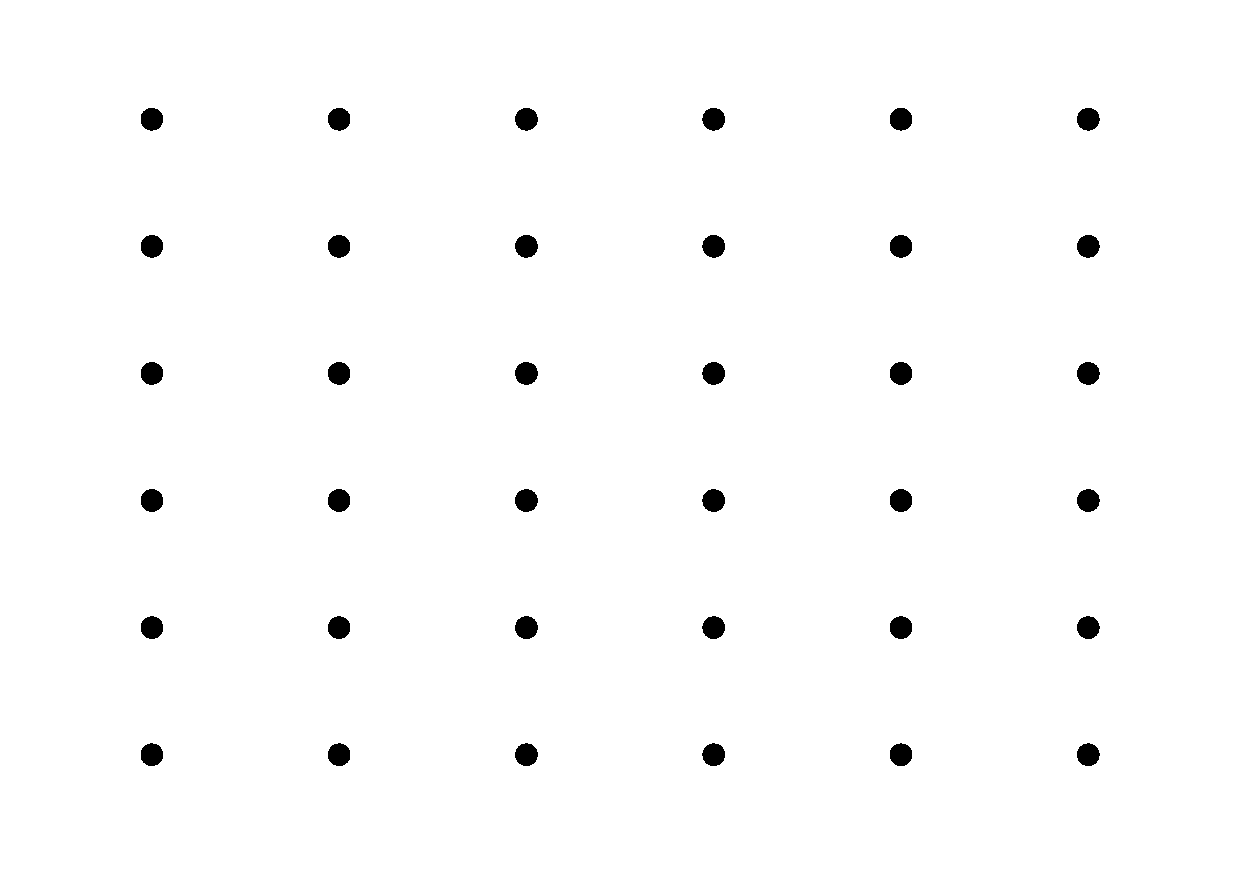
\includegraphics[width=\textwidth]{chp02_background/figures/gridpoints.pdf}
		\caption{An illustration of unresolved subgrid effects in a spatial discretisation.
			When a system is discretised, either from measurements or to numerically solve a model, processes between the grid points and no longer resolved or observed and yet can have a noticeable impact on the system.}
		\label{fig:subgrid_effects}
	\end{center}
\end{figure}


In particular, \citet{SuraEtAl_2005_MultiplicativeNoiseNonGaussianity} demonstrate that linear deterministic dynamics with multiplicative noise can be produce the non-Gaussian statistics that we observed in real systems.

\citet{DawsonPalmer_2015_SimulatingWeatherRegimes} showed through simulation studies that the performance of a high-resolution purely deterministic model can be matched by a lower-resolution stochastic model.


The mathematical formulation of stochastic parameterisation -- where model predictions are now random quantities -- lends itself naturally to data assimilation \citep{BudhirajaEtAl_2019_AssimilatingDataModels,Jazwinski_2014_StochasticProcessesFiltering,LawEtAl_2015_DataAssimilationMathematical,ReichCotter_2015_ProbabilisticForecastingBayesian}, where ongoing observations are combined with predictions from a model to produce an improved forecast.
Data assimilation provides a framework that can simultaneously account for uncertainty in the observations and the model itself.
It has been shown that stochastic parameterisation can improve the quality of forecasts in data assimilation schemes \citep{MitchellGottwald_2012_DataAssimilationSlow,HaEtAl_2015_ComparisonModelError}, and so these applications are an active error of research \citep[e.g.]{GottwaldHarlim_2013_RoleAdditiveMultiplicative}.

\td{Flow from here into the need for maths - justifications, proofs, etc.?}
There is an emerging need to bridge the gap between mathematicians working on developing stochastic theory and algorithms, and the scientists looking to apply this work to their respective fields.
In particular, \citet{BernerEtAl_2017_StochasticParameterizationNew} conclude that ``geoscientists are often unaware of mathematically rigorous results that can aid in the development of physically relevant parameterizations, [while] mathematicians often do not know about open issues in scientific applications that might be mathematically tractable''.


Although stochastic parameterisation is more common in the atmospheric modelling context, oceanography also suffers from the same trade-off between spatial resolution and accuracy of predictions.

In the context of a fluid, unresolved processes can be vortices, eddies and turbulence \citep{Griffa_1996_ApplicationsStochasticParticle}.

The mixing effect that these eddies have on the surrounding flow can be modelled with spatiotemporally-varying diffusion \citehere, which via the Fokker-Planck equation can be equivalently formulated as a stochastic differential equation with multiplicative noise.
The Lagrangian trajectories, incorporating these unresolved eddy effects, are then modelled as solutions to the stochastic differential equation.
Equivalently, through the Fokker-Planck equation we can consider the evolution of a passive tracer undergoing advection due to the deterministic drift and diffusion from both any natural diffusivity and the unresolved processes.
The probability density function that solves the Fokker-Planck equation can be instead thought of as a time-varying density (with the appropriate normalisation) of the tracer.
For instance, the Fokker-Planck equation has been used to model the transport of ??? with a stochastic framework \citehere.
Hence, understanding the evolution of solutions to a stochastic differential equation is valuable in oceanography, as a means of quantifying both observational error and unresolved subgrid processes.


There are several different methods for quantifying eddy diffusivity given either observed tracer data or a global ocean circulation model.

The simplest notion of eddy diffusivity is a defined by






A recent approach by \cite{YingEtAl_2019_BayesianInferenceOcean} uses Bayesian inference to estimate the eddy diffusivity tensor from observed Lagrangian tracer data, by numerically solving the Fokker-Planck equation to compute a likelihood function.


In summary, stochastic parameterisation



\section{Limitations of stochastic simulation and the need for further development}\label{sec:bkg_sim_limits}
The introduction of stochastic terms complicates both the analytical treatment of the model.
For example, we saw in \Cref{sec:sde_theory} that adding even additive and stationary\lb{Is this the right word?? I mean that \(\sigma\) is constant, with no time-dependency}\td{need to define additive versus multiplicative properly.} noise to an analytically solvable non-linear deterministic model can make exact solutions intractable.
Thus, across many applications the state of the art approach is to generate samples of the stochastic model and perform statistical inference.
For example, Monte-Carlo simulation is used across weather forecasting \citep{LeutbecherEtAl_2017_StochasticRepresentationsModel}, \td{something atmospheric} and \td{something oceanic}.

However, the most significant drawback of bulk stochastic simulation is the computational load.
In general, a large number of samples is required for convergent statistics and accurate inference, as discussed by \citet{Leutbecher_2019_EnsembleSizeHow}.
For a complex model, the computational load of computing a single realisation

The recent review by \citet{LeutbecherEtAl_2017_StochasticRepresentationsModel} highlights the need to develop computationally efficient schemes for quantifying stochasticity in weather and climate forecast models.


\td{Show the plateauing out that I am observing empirically when using a KDE . . . some literature on this?? This is a huge point to make}
For example, suppose that we intend on using the probabilistic forecast of our stochastic model in an inference scheme, such as in data assimilation in which model predictions are combined with ongoing observations to produce an improved forecast \cite[e.g.]{LawEtAl_2015_DataAssimilationMathematical,BudhirajaEtAl_2019_AssimilatingDataModels, ReichCotter_2015_ProbabilisticForecastingBayesian}.
This requires a probability density function or similar for our forecast, but in generating samples we initially only have a collection of finite discrete points.


The overall aim of this thesis is to address this problem, by developing characterisations of uncertainty and algorithms for approximating solution probability densities (as opposed to just generating samples) that are computationally efficient.
We aim to take advantage of the computational ease of generating solutions to a deterministic system (relative to taking many samples of a stochastic one).


The purpose of this example was to highlight the importance of accounting for measurement error and unresolved processes in a ; when the dynamics are complicated, then any uncertainty can have a significant impact on our inferences from the model, both quantitatively and qualitatively.



\section{Contributions of this thesis}


The contributions and structure of this thesis are as follows:
\begin{itemize}
	\item In \Cref{ch:linear_theory}, we address a slight deficiency in the \emph{theory} of SDE linearisations by providing an explicit bound on the strong error between a stochastic differential equation and an appropriate linearisation, capturing the impact of \emph{both} the ongoing linearisation and the choice of initial condition.
	      This builds upon previous studies of small-noise expansions \cite[e.g.]{Sanz-AlonsoStuart_2017_GaussianApproximationsSmall,Blagoveshchenskii_1962_DiffusionProcessesDepending,FreidlinWentzell_1998_RandomPerturbationsDynamical}, providing an direct proof in the multidimensional, fully-nonautonomous and multiplicative noise case, and an explicit expression for the bound while additionally extending these results to arbitrary initial conditions.
	      Using this bound, we provide conditions for the initialisation of the linearised equation.


	      % Be clear here. Two sentences - often lacks justification, OR when the justification is there, only additive or autonomous. "Albeit"
	      % The Gaussian distribution solving the linearised SDE appears in other literature and applications but often lacks justification \cite{Jazwinski_2014_StochasticProcessesFiltering, SarkkaSolin_2019_AppliedStochasticDifferential}.
	      % On the other hand, when the linearisation is justified, this is disregarding time-dependence in the coefficients and multiplicative noise \cite{Sanz-AlonsoStuart_2017_GaussianApproximationsSmall}.

	\item We provide, in a single place, a framework for characterising uncertainty in a system of ordinary differential equations via now justified linearisations, whereas previously these results were placed across \lb{I have not quite worded this the way I would like; }
	      The solution of the linearisation is expressed as an independent sum of the transformed initial condition and the ongoing
	      In \Cref{thm:limit_moments}, the mean and covariance of the linearisation are written in terms of the diffusion term and gradients of \emph{either} the drift term (as a pair of ordinary differential equations consistent with that arising elsewhere \cite[e.g.]{Jazwinski_2014_StochasticProcessesFiltering, Sanz-AlonsoStuart_2017_GaussianApproximationsSmall, SarkkaSolin_2019_AppliedStochasticDifferential, ArchambeauEtAl_2007_GaussianProcessApproximations}, or the flow map of the corresponding deterministic system.
	      The latter is an alternative characterisation that allows the Gaussian distribution to be computed \emph{entirely from the solution dynamics} of a deterministic model and specification of any multiplicative noise effects known prior.

	\item In \Cref{sec:theory_s2},

	\item In \Cref{sec:numerics}, we validate the results of \Cref{sec:theory} using stochastic simulations from a 2-dimensional model.
	      In particular, we demonstrate that the first four moments of the distance between the realisations and the Gaussian limit follow the predicted bound.
	      We also illustrate a key prediction from \Cref{sec:theory_s2}; that the computable covariance matrix of the Gaussian limit captures the time-evolution of uncertainty, even when the noise is multiplicative.

\end{itemize}
